%%%%%%%%%%%%%%%%%%%%%%%%%%%%%%%%%%%%%%%%%
% Compact Laboratory Book
% LaTeX Template
% Version 1.0 (4/6/12)
%
% This template has been downloaded from:
% http://www.LaTeXTemplates.com
%
% Original author:
% Joan Queralt Gil (http://phobos.xtec.cat/jqueralt) using the labbook class by
% Frank Kuster (http://www.ctan.org/tex-archive/macros/latex/contrib/labbook/)
%
% License:
% CC BY-NC-SA 3.0 (http://creativecommons.org/licenses/by-nc-sa/3.0/)
%
% Important note:
% This template requires the labbook.cls file to be in the same directory as the
% .tex file. The labbook.cls file provides the necessary structure to create the
% lab book.
%
% The \lipsum[#] commands throughout this template generate dummy text
% to fill the template out. These commands should all be removed when 
% writing lab book content.
%
% HOW TO USE THIS TEMPLATE 
% Each day in the lab consists of three main things:
%
% 1. LABDAY: The first thing to put is the \labday{} command with a date in 
% curly brackets, this will make a new section showing that you are working
% on a new day.
%
% 2. EXPERIMENT/SUBEXPERIMENT: Next you need to specify what 
% experiment(s) and subexperiment(s) you are working on with a 
% \experiment{} and \subexperiment{} commands with the experiment 
% shorthand in the curly brackets. The experiment shorthand is defined in the 
% 'DEFINITION OF EXPERIMENTS' section below, this means you can 
% say \experiment{pcr} and the actual text written to the PDF will be what 
% you set the 'pcr' experiment to be. If the experiment is a one off, you can 
% just write it in the bracket without creating a shorthand. Note: if you don't 
% want to have an experiment, just leave this out and it won't be printed.
%
% 3. CONTENT: Following the experiment is the content, i.e. what progress 
% you made on the experiment that day.
%
%%%%%%%%%%%%%%%%%%%%%%%%%%%%%%%%%%%%%%%%%

%----------------------------------------------------------------------------------------
%	PACKAGES AND OTHER DOCUMENT CONFIGURATIONS
%----------------------------------------------------------------------------------------                               

\documentclass[fontsize=11pt, % Document font size
paper=a4, % Document paper type
twoside, % Shifts odd pages to the left for easier reading when printed, can be changed to oneside
captions=tableheading,
index=totoc,
hyperref]{labbook}
\usepackage[framemethod=tikz]{mdframed}
\usepackage[bottom=10em]{geometry} % Reduces the whitespace at the bottom of the page so more text can fit

\usepackage[english]{babel} % English language
\usepackage{lipsum} % Used for inserting dummy 'Lorem ipsum' text into the template

\usepackage[utf8]{inputenc} % Uses the utf8 input encoding
\usepackage[T1]{fontenc} % Use 8-bit encoding that has 256 glyphs

\usepackage[osf]{mathpazo} % Palatino as the main font
\linespread{1.05}\selectfont % Palatino needs some extra spacing, here 5% extra
\usepackage[scaled=.88]{beramono} % Bera-Monospace
\usepackage[scaled=.86]{berasans} % Bera Sans-Serif

\usepackage{booktabs,array} % Packages for tables

\usepackage{amsmath} % For typesetting math
\usepackage{graphicx} % Required for including images
\usepackage{etoolbox}
\usepackage[norule]{footmisc} % Removes the horizontal rule from footnotes
\usepackage{lastpage} % Counts the number of pages of the document
\usepackage{shadowtext}
\usepackage{minted}
\usepackage[backend=biber,
style=authoryear-comp,
natbib=true,
]{biblatex}
\addbibresource{JNMansfieldCapstoneScholarshipPaper.bib}

\usepackage{setspace}
\usepackage{url}
\usetikzlibrary{shadows,arrows}
\tikzstyle{card}=[draw, fill=yellow!20, text width=6.0em, text centered,
minimum height=3.0em,drop shadow]
\tikzstyle{parent}=[circle, fill=green!60, text width=4.0em, text centered,
minimum height=3.0em,drop shadow]
\tikzstyle{child}=[circle, fill=green!20, text width=4.0em, text centered,
minimum height=3.0em,drop shadow]
\tikzstyle{childtwo}=[circle, fill=yellow!20, text width=4.0em, text centered,
minimum height=3.0em,drop shadow]

\addtokomafont{title}{\Huge\color{green!40!brown!80}} % Titles in custom blue color
\addtokomafont{chapter}{\color{green!40!brown!80}} % Lab dates in olive green
\addtokomafont{section}{\color{brown}} % Sections in sepia
\addtokomafont{pagehead}{\normalfont\sffamily\color{gray}} % Header text in gray and sans serif
\addtokomafont{caption}{\footnotesize\itshape} % Small italic font size for captions
\addtokomafont{captionlabel}{\upshape\bfseries} % Bold for caption labels
\addtokomafont{descriptionlabel}{\rmfamily}
\setcapwidth[r]{10cm} % Right align caption text
\setkomafont{footnote}{\sffamily} % Footnotes in sans serif

\deffootnote[4cm]{4cm}{1em}{\textsuperscript{\thefootnotemark}} % Indent footnotes to line up with text

\DeclareFixedFont{\textcap}{T1}{phv}{bx}{n}{1.5cm} % Font for main title: Helvetica 1.5 cm
\DeclareFixedFont{\textaut}{T1}{phv}{bx}{n}{0.8cm} % Font for author name: Helvetica 0.8 cm

\usepackage[nouppercase,headsepline]{scrpage2} % Provides headers and footers configuration
\pagestyle{scrheadings} % Print the headers and footers on all pages
\clearscrheadfoot % Clean old definitions if they exist

\automark[chapter]{chapter}
\ohead{\headmark} % Prints outer header

\setlength{\headheight}{25pt} % Makes the header take up a bit of extra space for aesthetics
\setheadsepline{.4pt} % Creates a thin rule under the header
\addtokomafont{headsepline}{\color{lightgray}} % Colors the rule under the header light gray

\ofoot[\normalfont\normalcolor{\thepage\ |\  \pageref{LastPage}}]{\normalfont\normalcolor{\thepage\ |\  \pageref{LastPage}}} % Creates an outer footer of: "current page | total pages"

% These lines make it so each new lab day directly follows the previous one i.e. does not start on a new page - comment them out to separate lab days on new pages
\makeatletter
\patchcmd{\addchap}{\if@openright\cleardoublepage\else\clearpage\fi}{\par}{}{}
\makeatother
\renewcommand*{\chapterpagestyle}{scrheadings}


% These lines make it so every figure and equation in the document is numbered consecutively rather than restarting at 1 for each lab day - comment them out to remove this behavior
\usepackage{chngcntr}
\counterwithout{figure}{labday}
\counterwithout{equation}{labday}

% Hyperlink configuration
\usepackage[
pdfauthor={}, % Your name for the author field in the PDF
pdftitle={Laboratory Journal}, % PDF title
pdfsubject={}, % PDF subject
bookmarksopen=true,
linktocpage=true,
pdfpagelabels=true,
plainpages=false,
colorlinks=true, % Turn off all coloring by changing this to false
bookmarks=true,
pdfview=FitB]{hyperref}

\usepackage[stretch=10]{microtype} % Slightly tweak font spacing for aesthetics

%\setlength\parindent{0pt} % Uncomment to remove all indentation from paragraphs

%----------------------------------------------------------------------------------------
%	DEFINITION OF EXPERIMENTS
%----------------------------------------------------------------------------------------

% Template: \newexperiment{<abbrev>}[<short form>]{<long form>}
% <abbrev> is the reference to use later in the .tex file in \experiment{}, the <short form> is only used in the table of contents and running title - it is optional, <long form> is what is printed in the lab book itself

\newexperiment{exp1}[Hello Dataface]{DataFace a Chunking Application for memory}
\newexperiment{exp2}[Connectionism]{Connectionism: neural networks}
\newexperiment{exp3}[Creating Objects]{Creating Objects}
\newexperiment{exp4}[Where is DataFace now?] {The current state of the DataFace application}
\newexperiment{exp5}[Appendices] {The current DataFace Source Code}


%----------------------------------------------------------------------------------------

\begin{document}

%----------------------------------------------------------------------------------------
%	TITLE PAGE
%----------------------------------------------------------------------------------------

\title{\textcap{\shadowtext{Regis University}\\
\textaut{\small{CS493}}	
\textaut{\small{Senior Capstone}}\\		
\textaut{\shadowtext{Scholarship Paper}}}
}

\author{

\includegraphics[scale=0.5]{android.png}\\
\textaut{\small{Intructor: Mr. Allan Rossi}}\\
\textaut{\small{Author: Mr. Jason N Mansfield}}\\ \\ % Your name
The Object Based Study Application % Your degree
}
\date{\today} % No date by default, add \today if you wish to include the publication date

\maketitle % Title page
\chapter*{abstract}
\begin{mdframed}[roundcorner=10pt,leftmargin=1, rightmargin=1, 
linecolor=green!40!brown!80,outerlinewidth=.9,
innerleftmargin=8,innertopmargin=8,innerbottommargin=8]
\begin{center}
\begin{minipage}[c]{0.5\textwidth}
The DataFace project is a Android application trying to become a Cheat Sheet or Flow Chart of sorts. This essay describes my attempt to create a application which provides a method for an individual to naturally memorize information using a technique similar to chunking. 
\end{minipage}
\end{center}
\end{mdframed}

\printindex
\tableofcontents % Table of contents
\newpage % Start lab look on a new page


\pagestyle{scrheadings} % Begin using headers

%----------------------------------------------------------------------------------------
%	LAB BOOK CONTENTS
%----------------------------------------------------------------------------------------

\labday{\today}
%-----------------------------------------
\experiment{exp1}
\begin{onehalfspace}
To some individuals memorizing trivial facts comes naturally. Unfortunately, for myself I have the tendency to lose any information I do not deem critical. I have arrived at the conclusion that the only way I can remember any trivial subject is by somehow organizing it in a way that gives it a purpose in my life. One particular approach which caught my attention is called Chunking~\citep{bor2012the}. An example of chunking might be the method you use to remember phone numbers. Memorizing telephone numbers is easy because you already use chucking as an approach:\\
\end{onehalfspace}
\begin{figure}[H]
\centering
\begin{tabular}{|c|c|c|c|}\hline
Calling code & Area Code & Central Office Code & Subscriber Number\\\hline
1 & 757 & 555 & 1234\\\hline
\end{tabular}
\caption{telephony}
\end{figure}
\begin{onehalfspace}
In the past few months I have been using various Flash Card programs, such as Anki, for memorizing trivial data. The problem I have experiencing is correlating items together. For example, I might be studying a piece of history in which a significant event happens in 1851; seven cards later an additional event happens in 1951. It was difficult for me to divide the two event when attempting to recall. However, in a cheat sheet, time line or other method all the dates are in front of you:
\end{onehalfspace}
\begin{figure}[H]
\centering
\begin{tikzpicture}
\node[card](card1){event one\\1851};
\node[card](card2)at (4,0) {event two\\1951};
\end{tikzpicture}
\caption{flashcards}
\end{figure}
\begin{onehalfspace}
Therefore, in an attempt to implement a chunking type approach, I have determined organizing objects together in a viewable format, is the best approach. This will allow the user to not only view the information, but all the related information to it. This approach will create an overall map of information, which allows the learner to connect and reinforce data objects together. If a learner cannot recall an event which happened in 1851, they may in fact remember that an event prior which happened in 1842, and an event that after happened in 1862. This grouping together will allow the learner to use surrounding data to isolate a correct answer. 
\end{onehalfspace}
\begin{figure}[H]
\centering
\begin{tikzpicture}
\node[parent](object1){Events};
\node[child](object2)at (-4,-2){event in 1842};
\node[child](object3)at (-1.5,-2) {event in 1851};
\node[child](object4)at (1.5,-2) {event in 1862};
\node[child](object5)at (4,-2) {event in 1951};
\draw [->](object1) -- (object2);
\draw [->](object1) -- (object3);
\draw [->](object1) -- (object4);
\draw [->](object1) -- (object5);
\end{tikzpicture}
\caption{objects}
\end{figure}
\experiment{exp2}
\begin{onehalfspace}
	To be perfectly honest when I began this project I had no backing information to believe my object based approach was relevant. However, as I began to explore I discovered that I'm not the only one to hold this view. Similar to an Object based approach Connectionism theorists believe the brains neural network uses a large number of units which are joined together~\citep{sep-connectionism}.
\end{onehalfspace}
\begin{figure}[H]
\centering
\begin{tikzpicture}
	\node[parent](parent1)at (0,0){Input Unit};
\node[parent](parent2)at (0,-2){Input Unit};
\node[parent](parent3)at (0,-4){Input Unit};
\node[parent](parent4)at (0,-6){Input Unit};
\node[parent](parent5)at (0,-8){Input Unit};
\node[parent](parent6)at (0,-10){Input Unit};
\node[parent](parent7)at (0,-12){Input Unit};

\node[child](object2)at (5,0){Hidden Units};
\node[child](object3)at (5,-4){Hidden Units}; 
\node[child](object4)at (5,-8) {Hidden Units};
\node[child](object5)at (5,-12) {Hidden Units};

\node[childtwo](child)at (10,-2){Output Units}; 
\node[childtwo](child2)at (10,-6){Output Units}; 
\node[childtwo](child3)at (10,-10){Output Units}; 


\draw [->](parent1) -- (object2);
\draw [->](parent1) -- (object3);
\draw [->](parent1) -- (object4);
\draw [->](parent1) -- (object5);

\draw [->](object4) -- (child);
\draw [->](object4) -- (child2);
\draw [->](object4) -- (child3);
\end{tikzpicture}
\caption{simple neural net}
\end{figure}
\begin{onehalfspace}
	The object based approach is of course not nearly as intricate as the brains supposed neural network, but I do believe this example drives home the point of using connections. Unlike, episodic memory which is obtained by personal or experiential memory; semantic memory is conceptual and based on learned facts~\citep{sep-memory}. The key is to create enough connections with factual data objects to pass the information from semantic to declarative memory for future recall.  
\end{onehalfspace}
\experiment{exp3}
\begin{onehalfspace}
Using a method similar to chunking the DataFace application strives to use small pieces of larger information. The DataFace format allows the creation of a parent Object which can then be populated with child items:
\end{onehalfspace}
\begin{figure}[H]
\centering
\begin{tikzpicture}
\node[parent](object1){Parent Object};
\node[child](object2)at (-4,-2){child object};
\node[child](object3)at (-1.5,-2) {child object};
\node[child](object4)at (1.5,-2) {child object};
\node[child](object5)at (4,-2) {child object};
\draw [->](object1) -- (object2);
\draw [->](object1) -- (object3);
\draw [->](object1) -- (object4);
\draw [->](object1) -- (object5);
\end{tikzpicture}
\caption{Parent and child objects}
\end{figure}
\begin{onehalfspace}
	The idea behind this object based application is similar to a flow chart in that the child items can all be seen simultaneously. Additionally, there should be a way to also correlate all the parent objects as well. I selected a Android based platform due to it open platform allowing me the ability to freely share the final product. Using the Android platform also allows outside users an easy way to use and share the product if not contribute to its development. Future development should include enhancing the graphical view of the child objects as previously described, add a mathematical markup language such as LaTeX or MathML, and the ability to parse in data through text documents in formats such as CSV or XML. The first steps of creating a SQLite~\citep{sqlite} database which can manage both Parent and Child objects with a view has been accomplished. However, I am far from satisfied with the child items in a ListView~\citep{ListView} type format. Once I can create a Layout and View which allows all the child items to be viewed at once, possibly a modified GridView~\citep{gridview}, I feel this particular application will have usefulness. 
\end{onehalfspace}
\experiment{exp4}
\begin{onehalfspace}
Although, the DataFace application has not reached a mature level, the structure seems to be intact. The parent objects allow for a Title and a short description. The child items are identical with the exception that they are encapsulated within the parent object. This was the first real application I have created using both Java and the Android API, as well as using SQLite3. I was able to research and implement the following items into my application:
\end{onehalfspace}
\begin{description}
\item[Activities] I discover how to communicate between activities using intents~\citep{Intent} and bundles~\citep{Bundle}.
\item[SimpleCursorAdapter] The SimpleCursorAdapter~\citep{SimpleCursorAdapter} was one adapter that I used during development, and is the remaining adapter now due to its ability to take SQLite column data and create a proper ListView.
\item[Constructors] Although, I have created constructors~\citep{Ravi} before it was not for a useful purpose. DataFace contains two constructors, one for the Parent object and One for the Child Objects.
\item[SQLite3] SQLite3 matched with Android makes an excellent environment for development. I have created web applications before, but creating this Java based application using sqlite3~\citep{vogella} on Android was by far the most rewarding experience.
\end{description}
\experiment{exp5}
\begin{onehalfspace}
	The education I have received at Regis University has certainly opened my eyes to new possibilities. Through classes such as CS375 Advanced Programming and Algorithms, and MT320 Introduction to Discrete Mathematics; I have learned to have a unprejudiced view towards certain programing languages, but instead concern myself with the underlying logic. My favorite classes MT360A and MT360B Calculus I and II, prepared me for the discipline I needed to take a real world problem and break it down into a solution. Clearly, the knowledge I gained taking CS442 Database programming was helpful during the development of DataFace with its use of SQLite3. The DataFace application still needs quite a bit of upgrading and implementation. A large issue with this particular project was my limited knowledge in Android development. Although, CS434 Object Oriented Programming using Java was an excellent class, I was a little rusty and the Android environment has some big twists such as the Actvities, Intents and so forth. In retrospect I wish I had spent less time on creating a Fragment view and simply understanding the basics of an Activity. I began the project believing the implementation of a Fragment~\citep{fragments} was critical.  Overall, I was able to accomplish what I thought could be done by this time. I'm fairly certain there are still quite a few beginner development flaws within the application which will require re-writing over time. I currently have two sqlite databases being used due to a semi-stable delete function. Eventually, there will likely only be a single database with two tables. The more I learn about managing the sqlite database using the Android API the better my application will become. Additionally, as previously mentioned a GridView might just be the trick needed for the child views but only time and future efforts will make that determination. This was a tremendously satisfying project for me and I am excited to see what I can accomplish in the future with the knowledge handed to me by my Instructors at Regis. 
\end{onehalfspace}
\clearpage
\chapter*{Appendix}
\begin{mdframed}[roundcorner=10pt,leftmargin=1, rightmargin=1, 
linecolor=green!40!brown!80,outerlinewidth=.9,
innerleftmargin=8,innertopmargin=8,innerbottommargin=8]
\begin{center}
\begin{minipage}[c]{1.0\textwidth}
To view the current DataFace project you may download and use the latest APK to use on your Android based device: \href{https://github.com/trentonknight/DataFaceProject/blob/master/DataFace/build/apk/DataFace-release-unsigned.apk?raw=true}{Dataface-release-unsigned.apk}
\end{minipage}
\end{center}
\end{mdframed}
\begin{mdframed}[roundcorner=10pt,leftmargin=1, rightmargin=1, 
linecolor=green!40!brown!80,outerlinewidth=.9,
innerleftmargin=8,innertopmargin=8,innerbottommargin=8]
\begin{center}
\begin{minipage}[c]{1.0\textwidth}
To view the latest development source code of this product, please take a look at the online GitHub repository: \href{https://github.com/trentonknight/DataFaceProject}{DataFaceProject}
\end{minipage}
\end{center}
\end{mdframed}
\begin{mdframed}[roundcorner=10pt,leftmargin=1, rightmargin=1, 
linecolor=green!40!brown!80,outerlinewidth=.9,
innerleftmargin=8,innertopmargin=8,innerbottommargin=8]
\begin{center}
\begin{minipage}[c]{1.0\textwidth}
To clone this project using git:\\ git~clone~\href{https://github.com/trentonknight/DataFaceProject.git}{https://github.com/trentonknight/DataFaceProject.git}
\end{minipage}
\end{center}
\end{mdframed}
\begin{mdframed}[roundcorner=10pt,leftmargin=1, rightmargin=1, 
linecolor=green!40!brown!80,outerlinewidth=.9,
innerleftmargin=8,innertopmargin=8,innerbottommargin=8]
\begin{center}
\begin{minipage}[c]{1.0\textwidth}
To comment or see status updates on this project view the wiki here: \href{https://github.com/trentonknight/DataFaceProject/wiki/DataFace:-An-attempt-to-create-a-Object-based-learning-tool.}{DataFace: An attempt to create a Object based learning tool.}
\end{minipage}
\end{center}
\end{mdframed}
\clearpage
\printbibliography

\end{document}
